\section{The \thelibos{} Architecture}


The \libos{} of \graphene{}, or 
\thelibos{},
is a single library to be loaded beneath a Linux application,
as a compatible layer between
Linux \linuxapis{} and \thehostabi{}.
The purpose of \thelibos{} is to reuse an unmodified Linux application
upon an incompatible host OS or hardware.
%to support compatible OS features.
%for exporting compatible features.
An unmodified Linux application is built with the assumption of running on a Linux kernel or equivalent.
A Linux kernel
has exported a set of idiosyncratic features and characteristics,
or {\bf personality},
which an unmodified Linux application depends on.
%In order to reuse an unmodified Linux application
%on an incompatible host,
\thelibos{} takes the role of reproducing the Linux personality,
and is equivalent to a guest Linux kernel
over various host options.
%using \thehostabi{} exported by the host OS and PAL.
%The purpose of \thelibos{}
%is to resue an unmodified Linux application,
%by combining with a PAL and a host OS to behave as an equivalence of a Linux kernel. 
%%which is developed upon the assumption of running on a Linux kernel or equivalent.
%The main purpose of \thelibos{} is to reproduce
%the idiosyncratic features and behaviors of Linux,
%or the {\bf Linux personality},
%to resurrect Linux applications upon incompatible
%host OSes or hardware.
\graphene{} develops \thelibos{} as an ELF dynamic library (i.e., \code{\tt libLinux.so}),
loadable and linkable by a PAL.
%to be loaded on a host by the corresponding PAL.
%at the beginning of a \picoproc{}.


A key component of \thelibos{}
is a Linux system call table, which redirects \linuxapis{} from a Linux application to functions in \thelibos{}.
%a key Linux kernel component applications. 
%that \thelibos{} implements is the Linux system call table.
%For Linux and similar OSes,
A system call table is a primary entry point of a Linux kernel.
Each entry of the system call table
points to the kernel implementation of a Linux API related with a \linuxapi{} number (e.g., \code{NR\_open}).
%and triggers in-kernel operations for servicing requests from applications.
%and defines the interaction between applications and kernel.
\graphene{} moves the Linux system call table into \thelibos{},
and implements a number of \linuxapi{} handlers in the user space.
%The system call table in \thelibos{} contains a number of \linuxapi{} handlers,
Each \linuxapi{} handler emulates
individual \linuxapi{} that \graphene{} supports;
\graphene{} develops each handler
based on either a known specification, % known by the Linux application developers,
mostly described by a Linux manpage~\cite{linux-man-syscall},
or bug-for-bug behaviors
observed in a real Linux kernel.
For example, \syscall{rt\_sigaction} is partially documented
in the corresponding Linux manpage, and \thelibos{} implements the \linuxapi{} by mimicking the Linux kernel.
\graphene{} grows the functionality of \thelibos{}
primarily by extending the guest-level Linux system call table
with more complete \linuxapi{} implementation.

%Otherwise, for a few \linuxapis{} whose behaviors
%are not clearly defined by the Linux manpages,
%such as \syscall{rt\_sigaction},
%the \linuxapi{} handlers mimic the bug-for-bug behaviors of an actual Linux kernel.
%A continuing goal in \graphene{} is
%to extend \thelibos{} with more complete \linuxapi{} handlers.


%grow the functionality of \thelibos{},
%by extending the system call table with more complete handlers.




%The development of \linuxapi{} handlers in \thelibos{}
%is equivalent to implementing the specifications described in the Linux man pages~\cite{linux-man-syscall},
%including the valid inputs to each \linuxapi{},
%as well as the expected outcome.


%\paragraph{Implementing Linux Personality.} 
%\fixmedp{Revisit the logical flow of these paragraphs}
\Thelibos{} currently implements \graphenesyscallnum{} \linuxapis{},
and demonstrates 
the sufficiency of running applications ranging from servers to command-line applications.
For reference,
a relatively recent Linux kernel contains more than three hundred \linuxapis{}, including a long tail of infrequently-used \linuxapis{}.
%upon \thehostabi{}. % to interact with the host.
%Among the whole Linux \linuxapi{} table,
%A Linux kernel exports a long tail of infrequently-used \linuxapis{}.
%For reference, the Linux \linuxversion{} kernel exports \linuxsyscallnum{} \linuxapis{}.
A study of the Linux \linuxapi{} usage~\cite{tsai16apistudy}
indicates that only forty \linuxapis{} are indispensable to every applications available in the Ubuntu official repositories.
%The study also shows that
In the meantime, more than a hundred \linuxapis{} are used by only a single application,
or no application at all.
The development of \thelibos{} begins with
implementing twelve basic \linuxapis{} needed for running a ``hello world'' application,
such as \syscall{read}, \syscall{write}, and \syscall{open},
and then gradually grows the count of \linuxapis{}.
%for each new application introduced to run on \graphene{}.
As the count of \linuxapis{} continues to grow,
each time \thelibos{} is tested against a new application, the number of \linuxapis{} that need to be added
has dropped.
%Based on the types of applications priorized in \graphene{}, including servers, command-line programs, and language runtimes, some \linuxapis{} to be more important %for reusing the applications
%than the others. % \linuxapis{}.
According to the usage of each \linuxapi{} in applications,
developers can prioritize the popular \linuxapis{}, over other \linuxapis{} that are either unpopular among applications, or only used by administrative tools such as \code{reboot} or \code{ifconfig}.
\thelibos{} demonstrates that
\thehostabi{} is sufficient for implementing
a significant subset of the Linux \linuxapis{} to run
a representative sample of applications.


%The current \thelibos{} implementation
%includes a set of high-valued Linux \linuxapis{} for the types of applications
%that \graphene{} has targeted,
%including servers, command-line programs, and runtimes.
%The remaning \linuxapis{} may require extending \thehostabi{} with more privileged abstractions,
%including administrative operations
%and host-specific features.
%\thelibos{} demonstrates that \thehostabi{} is sufficient
%for exporting the host abstractions, to support a representative sample of Linux applications.

%such as memory sharing, scheduler configuration, and NUMA (non-uniform memory architecture) support.


%Linux exports a very long tail of infrequently-used \linuxapis{}.
%applications.




%An analysis indicates roughly 100 additional calls that can be implemented
%with the existing \pal{} ABI and coordination framework, less than 10 administrative calls that will not make sense to expose to 
%an application, such as loading a kernel module or rebooting the system, and roughly 54 that will require 
%\pal{} extensions to meaningfully implement, such as controlling scheduling,
%NUMA placement, I/O privilege, and shared memory.
%In the last category of system calls, the degree to which actual host details should be exported versus emulated is debatable.

%We believe represent the most commonly used system calls.
%When an application requests a call or argument that {\tt libLinux.so} does not implement,
%the picoprocess exits with a distinct error message. 
%Each time we have tested \graphene{} with a new application, the number of extra system calls
%required has dropped---most recently we only added 4 calls
%(namely, epoll\_create, epoll\_wait, semget and semop)
%to support the Apache web server.
%Thus, we believe \graphene{} implements a representative sample of Linux calls.

%such as {\tt sched\_setparam}, which manipulates scheduler-specific
%parameters or 
%{\tt uselib}, which has been abandoned 
%in {\tt glibc} version 2 in favor of a user-space dynamic linker.
%We do not plan to implement administrative interfaces, such as {\tt reboot}.
%The growth in the set of supported system calls has been driven by 
%the requirements of new applications we use to exercise \graphene{}, and has been 
%slowing considerably over time.



\subsection{\Linuxapi{} redirection}


\thelibos{} transparently intercepts \linuxapis{} in a Linux application. In a Linux kernel, a \linuxapi{} interrupt handler is assigned
to trigger the kernel operations,
whenever the application executes
a ``\assembly{syscall}'' or ``\assembly{int \$80}'' instruction.
The handler
performs a context switch from the application to kernel,
and redirects \linuxapi{} arguments to the kernel routine which services the requested \linuxapi{}.
%based on a kernel convention agreed by applications and Linux kernels.
\thelibos{} intercepts the \linuxapis{}
from an unmodified Linux executable or library, and redirects
to the system call table implemented inside \thelibos{}.
%intercepts the \linuxapis{}
%in an executable or library binary, and redirect the \linuxapis{}
%to the \linuxapi{} handlers inside \thelibos{}.
%\thelibos{} implements the callback functions for a subset of the Linux \linuxapis{}.
%For reference, Linux kernel \linuxversion{}
%has defined \linuxsyscallnum{} \linuxapis{} in total.


In normal cases,
\thelibos{} can redirect \linuxapis{} from an unmodified Linux application
using a modified C library (\libc{}).
%from an unmodified Linux application.
Most Linux executables and libraries avoid invoking \linuxapis{} directly,
but use \libc{} functions as wrappers to \linuxapis{}.
%which internally execute ``\code{syscall}'' or ``\code{int \$80}'' instructions.
%an executable or library in Linux and similar OSes invokes \linuxapis{} through \libc{},
%instead of directly containing the \code{syscall} instructions.
%The \libc{}
%contains a large set of \linuxapi{} wrappers,
%which encapsulate direct \linuxapis{} to the kernel as functions.
For example, the \libc{} function \funcname{read} is a wrapper to the \syscall{read} \linuxapi{},
which internally executes
the \assembly{syscall} instruction.
% that bares the same name and definition.
By defualt, \thelibos{} uses a modified
{\bf GNU C library (\glibc{})}~\cite{glibc},
since \glibc{} is compatible against most Linux applications released by Ubuntu. % are compatible against \glibc{}.
%which is compatible against most of the Linux applications released for Ubuntu.
%Other \libc{} variants, ,
%which are either fully or partially compatible with \glibc{},
%can be also modified to redirect \linuxapis{} to \thelibos{}.
%are alternatives upon \thelibos{} as long as they are modified for .
\graphene{} can also use other \libc{} variants,
such as \projname{uClibc}~\cite{uclibc} and \projname{musl}~\cite{musl},
if the application requires less \libc{} functionality.
%\graphene{} demonstrates that 
%are also demonstrated
%to be acceptable alternatives,
%with slight modification for \linuxapi{} redirection.




\graphene{} restricts the modification in \glibc{}
to up to \gipclines{} lines of code.
The C source code in \glibc{} consistently uses a platform-independent macro,
%referenced a single macro called
\funcname{INLINE\_SYSCALL},
to invoke \linuxapis{} to the kernel.
%when it needs to invoke a \linuxapi{}.
\funcname{INLINE\_SYSCALL} contains a piece of assembly code
that copies \linuxapi{} number and arguments to registers,
and then uses \assembly{syscall} to enter a Linux kernel.
\graphene{} modifies \funcname{INLINE\_SYSCALL}
to redirect a \linuxapi{} to
an entry point of \thelibos{} called \funcname{syscalldb}.
\funcname{syscalldb} saves the current register state, similar to a context switch,
and then
calls the \linuxapi{} handler
indicated by the \linuxapi{} number.
%, to trigger operations inside \thelibos{}.
For assembly code in \glibc{},
\graphene{} replaces each \code{syscall} instruction with
a dynamic call to
\funcname{syscalldb}, given the address of \funcname{syscalldb} is dynamically determined.
Figure~\ref{fig:libos:syscall-redirection} summarizes the mechanism of \linuxapi{} redirection.
%to \thelibos{}.


\begin{figure}[t!]
\centering
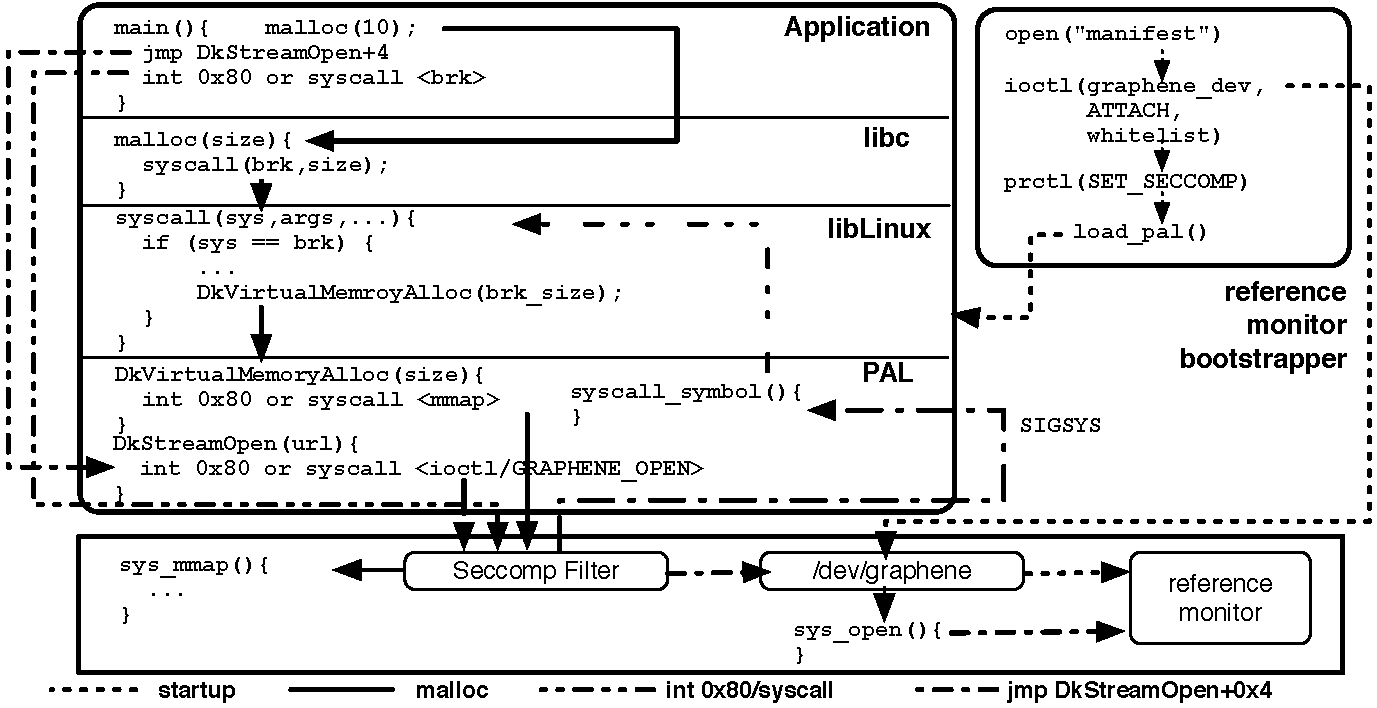
\includegraphics[width=\linewidth]{syscall-redirection.pdf}
\footnotesize
\caption{System call redirection for \thelibos{}.
In the normal case (first line of {\tt main}), {\tt malloc} is invoked causing the invocation of {\tt brk} ({\tt libLinux}) and {\tt mmap} in the \pal{}. In the second line, the application jumps to an address in \pal{}, which is permissible.
Files are accessed through {\tt ioctl} to {\tt /dev/graphene} and checked by reference monitor.
The third line invokes {\tt brk} with an {\tt int} instruction, which is redirected to the {\tt libLinux} function.}
\label{fig:libos:syscall-redirection}
\end{figure}


\graphene{} modifies several \glibc{} libraries with individual purposes,
%When using \graphene{}, an application must be deployed with the modified \libc{} libraries,
including \code{ld.so}, \code{libc.so}, \libpthread{}, and \libdl{}.
\Glibc{} partitions its code into separate libraries to reduce the binary sizes
loaded by each application.
%Despite that \glibc{} has partitioned its code into separate libraries,
\graphene{} only modifies the libraries which contains direct \linuxapis{} (i.e., \assembly{syscall} instructions).
%not every libraries of \glibc{} need to be modified for \linuxapi{} redirection.
%Only \code{libc.so}, \libpthread{}, and \libdl{} have included \code{syscall} instructions,
%and thus have to be modified for \graphene{}.
Other \libc{} libraries, such as \code{libm.so},
never directly invoke \linuxapis{} and only rely on 
existing \libc{} functions;
therefore, \graphene{} leaves \code{libm.so} and other similar \libc{} libraries unmodified.



\paragraph{Hard-coded \linuxapis{}.}
A static binary, or a platform-dependent application, may contain hard-coded \assembly{syscall} instructions
that cannot be redirected by a modified \libc{}.
Some application developers choose to statically link an executable against \libc{},
as a static binary with hard-coded \linuxapis{}. %\code{syscall} instructions.
Other application developers may program an application---usually a language runtime (e.g., go runtime) or system software (e.g., \projname{busybox})---with assembly code that directly invokes
platform-depenedent,
rare \linuxapis{} that are not wrapped by \libc{} functions.
%one of the \linuxapi{} wrappers in \libc{}, or \funcname{syscall}.
%As a result, a ELF binary may contain hard-coded \assembly{syscall} instructions.
%Either way leads to hard-coding \code{syscall} instructions in the ELF binaries.
Because modified \glibc{} does not redirect hard-coded \linuxapis{},
the \linuxapis{}
trigger context-switching into the host kernel,
causing security and compatibility issues as
exposing unauthorized, or unsynchronized host resources and states to the application.



\thelibos{} depends on host-level \linuxapi{} restriction to redirect hard-coded \linuxapis{}.
%to prevent \linuxapis{} from anywhere other than a PAL.
A direct \linuxapi{} traps into the host kernel,
unless the host has virtualized the interrupt handler to the \libos{}.
\graphene{} depends on each host to
detect unauthorized \linuxapis{} either from a wrong code location or with an unexpected \linuxapi{} number.
On Linux or a similar OS, the PAL can install a \linuxapi{} filter,
such as SECCOMP filter~\cite{seccomp}.
On some architecture, there are architectural limitation;
for example, SGX forbids \linuxapis{} inside an enclave and triggers an exception for an in-enclave \linuxapi{}.
%\code{syscall} instructions
%(e.g., SGX restriction).
%The details of the \linuxapi{} restriction mechanisms are discussed in
%\fixme{update labels}
%Section~\ref{sec:linux:syscall} and Section~\ref{sec:sgx:syscall}.
\thehostabi{} specifies that the host captures unauthorizes \linuxapis{}
and redirects to an exception handler (set up by \palcall{ExceptionSetHandler}).
%If a binary makes an illegal \linuxapi{},
%the host-level \linuxapi{} restriction will trigger an \code{ILLEGAL} exception
%at \thehostabi{},
%and thus the \linuxapi{} is redirected by an exception handler
%assigned by \thelibos{}.
The exception handler 
retrieves the \linuxapi{} number and arguments
from the saved context,
runs the \linuxapi{} handler,
and eventually pushes the return value back to the saved context. %\code{RAX} register.


Redirecting \linuxapis{} based on exceptions
can be expensive,
due to the overhead of context-switching between the host and guest.
Whenever an application invokes a direct \linuxapi{},
it traps into the host kernel, and then returns to the \libos{} to handle the \linuxapi{}.
Therefore, the process of redirecting a \linuxapi{} includes at least two times of context-switching, which can take up to microseconds.
To bypass the overhead,
\thelibos{} can 
rewrite the binary at run-time to redirect the hard-coded \linuxapis{};
%use {\bf binary translation} to modify the hard-coded \code{syscall} instructions;
\thelibos{} can
either scan-and-rewrites the whole binary at loading time,
or rewrites a single \assembly{SYSCALL} instruction in the exception handler.
%binary translation
%can be triggered when a host-level exception is raised
%for an illegal \linuxapi{},
%to optimize consecutive \linuxapi{} invocation at the same location.
%\thelibos{} can also perform a full scan in application binaries
%to spot and modify hard-code \code{syscall} instructions.
\graphene{} leaves the implementation of binary rewriting
as future work.


